
\chapter{SOLUTION}

\section{Overview}

I propose a new DNS system for Tor hidden services, which I am calling EsgalDNS. \emph{Esgal} is a Sindarin Elvish noun from the works of J.R.R Tolkien, meaning ``veil'' or ``cover that hides''.\cite{SindarinDict} EsgalDNS is a distributed DNS system embedded within the Tor network on top of the existing Tor hidden service infrastructure. EsgalDNS shares some design principles with Namecoin and its domain names resemble traditional domain names on the clearnet. At a high level, the system is powered at any given time by a randomly-chosen subset of Tor nodes, whose primary responsibilities are to receive new DNS records from hidden service operators, propagate the records to all parties, and save the records in a main long-term data structure. Other Tor nodes may mirror this data structure, distributing the load and responsibilities to many Tor nodes. The system supports a variety of command and control operations including Create, Domain Query, Onion Query, Modify, Move, Renew, and Delete.

% modify, move, and renew all renew, delete instantly cancels the record

\section{Cryptographic Primitives}

Our system makes use of cryptographic hash algorithms, digital signatures, proof-of-work, and a pseudorandom number generator. As the cryptographic data within our system must persist for many years to come, we select well-established algorithms that we predict will remain strong against cryptographic analysis in the immediate future.

\begin{itemize}
	\item Hash function - We choose SHA-384 for most applications for its greater resistance to preimage, collision, and pseudo-collision attacks over SHA-256, which is itself significantly stronger than Tor's default hidden service hash algorithm, SHA-1. Like SHA-512, SHA-384 requires 80 rounds but its output is truncated to 48 bytes rather than the full 64, which saves space.
	\item Digital signatures - Our default method is EMSA-PSS, (EMSA4) a probabilistic signature scheme defined by PKCS1 v2.1 and republished in 2003's RFC 3447, using a Tor node's 1024-bit RSA key with the SHA-384 digest to form the signature appendix. For signatures inside our proof-of-work scheme, we rely on EMSA-PKCS1-v1.5, (EMSA3) defined by 1998's RFC 2315. In contrast to EMSA-PSS, its deterministic nature prevents hidden service operators from bypassing the proof-of-work and brute-forcing the signature to validate the record.
	\item Proof-of-work - We select scrypt, a password-based key derivation function which is notable for its large memory and CPU requirements during its operation. The scrypt function provides significantly greater resistance to custom hardware attacks and massively parallel computation primarily due to its memory requirements. This limits attackers to the same software implementation and asymptotic cost as legitimate users.\cite{percival2009stronger} We choose scrypt because of these advantages over other key derivation functions such as SHA-256 or PBKDF2.
	\item Pseudorandom number generation - In applications that require pseudorandom numbers from a known seed, we use the Mersenne Twister generator. In all instances the Mersenne Twister is initialized from the output of a hash algorithm, negating the generator's weakness of producing substandard random output from certain types of initial seeds.
\end{itemize}

We use the JSON format to encode records and databases of records. JSON is significantly more compact than XML, but retains readability. Its support of basic primitive types is highly applicable to our needs. Additionally, we consider the JSON format safer than byte-level encoding.

\section{Participants}

\begin{figure}[htbp]
	\centering
	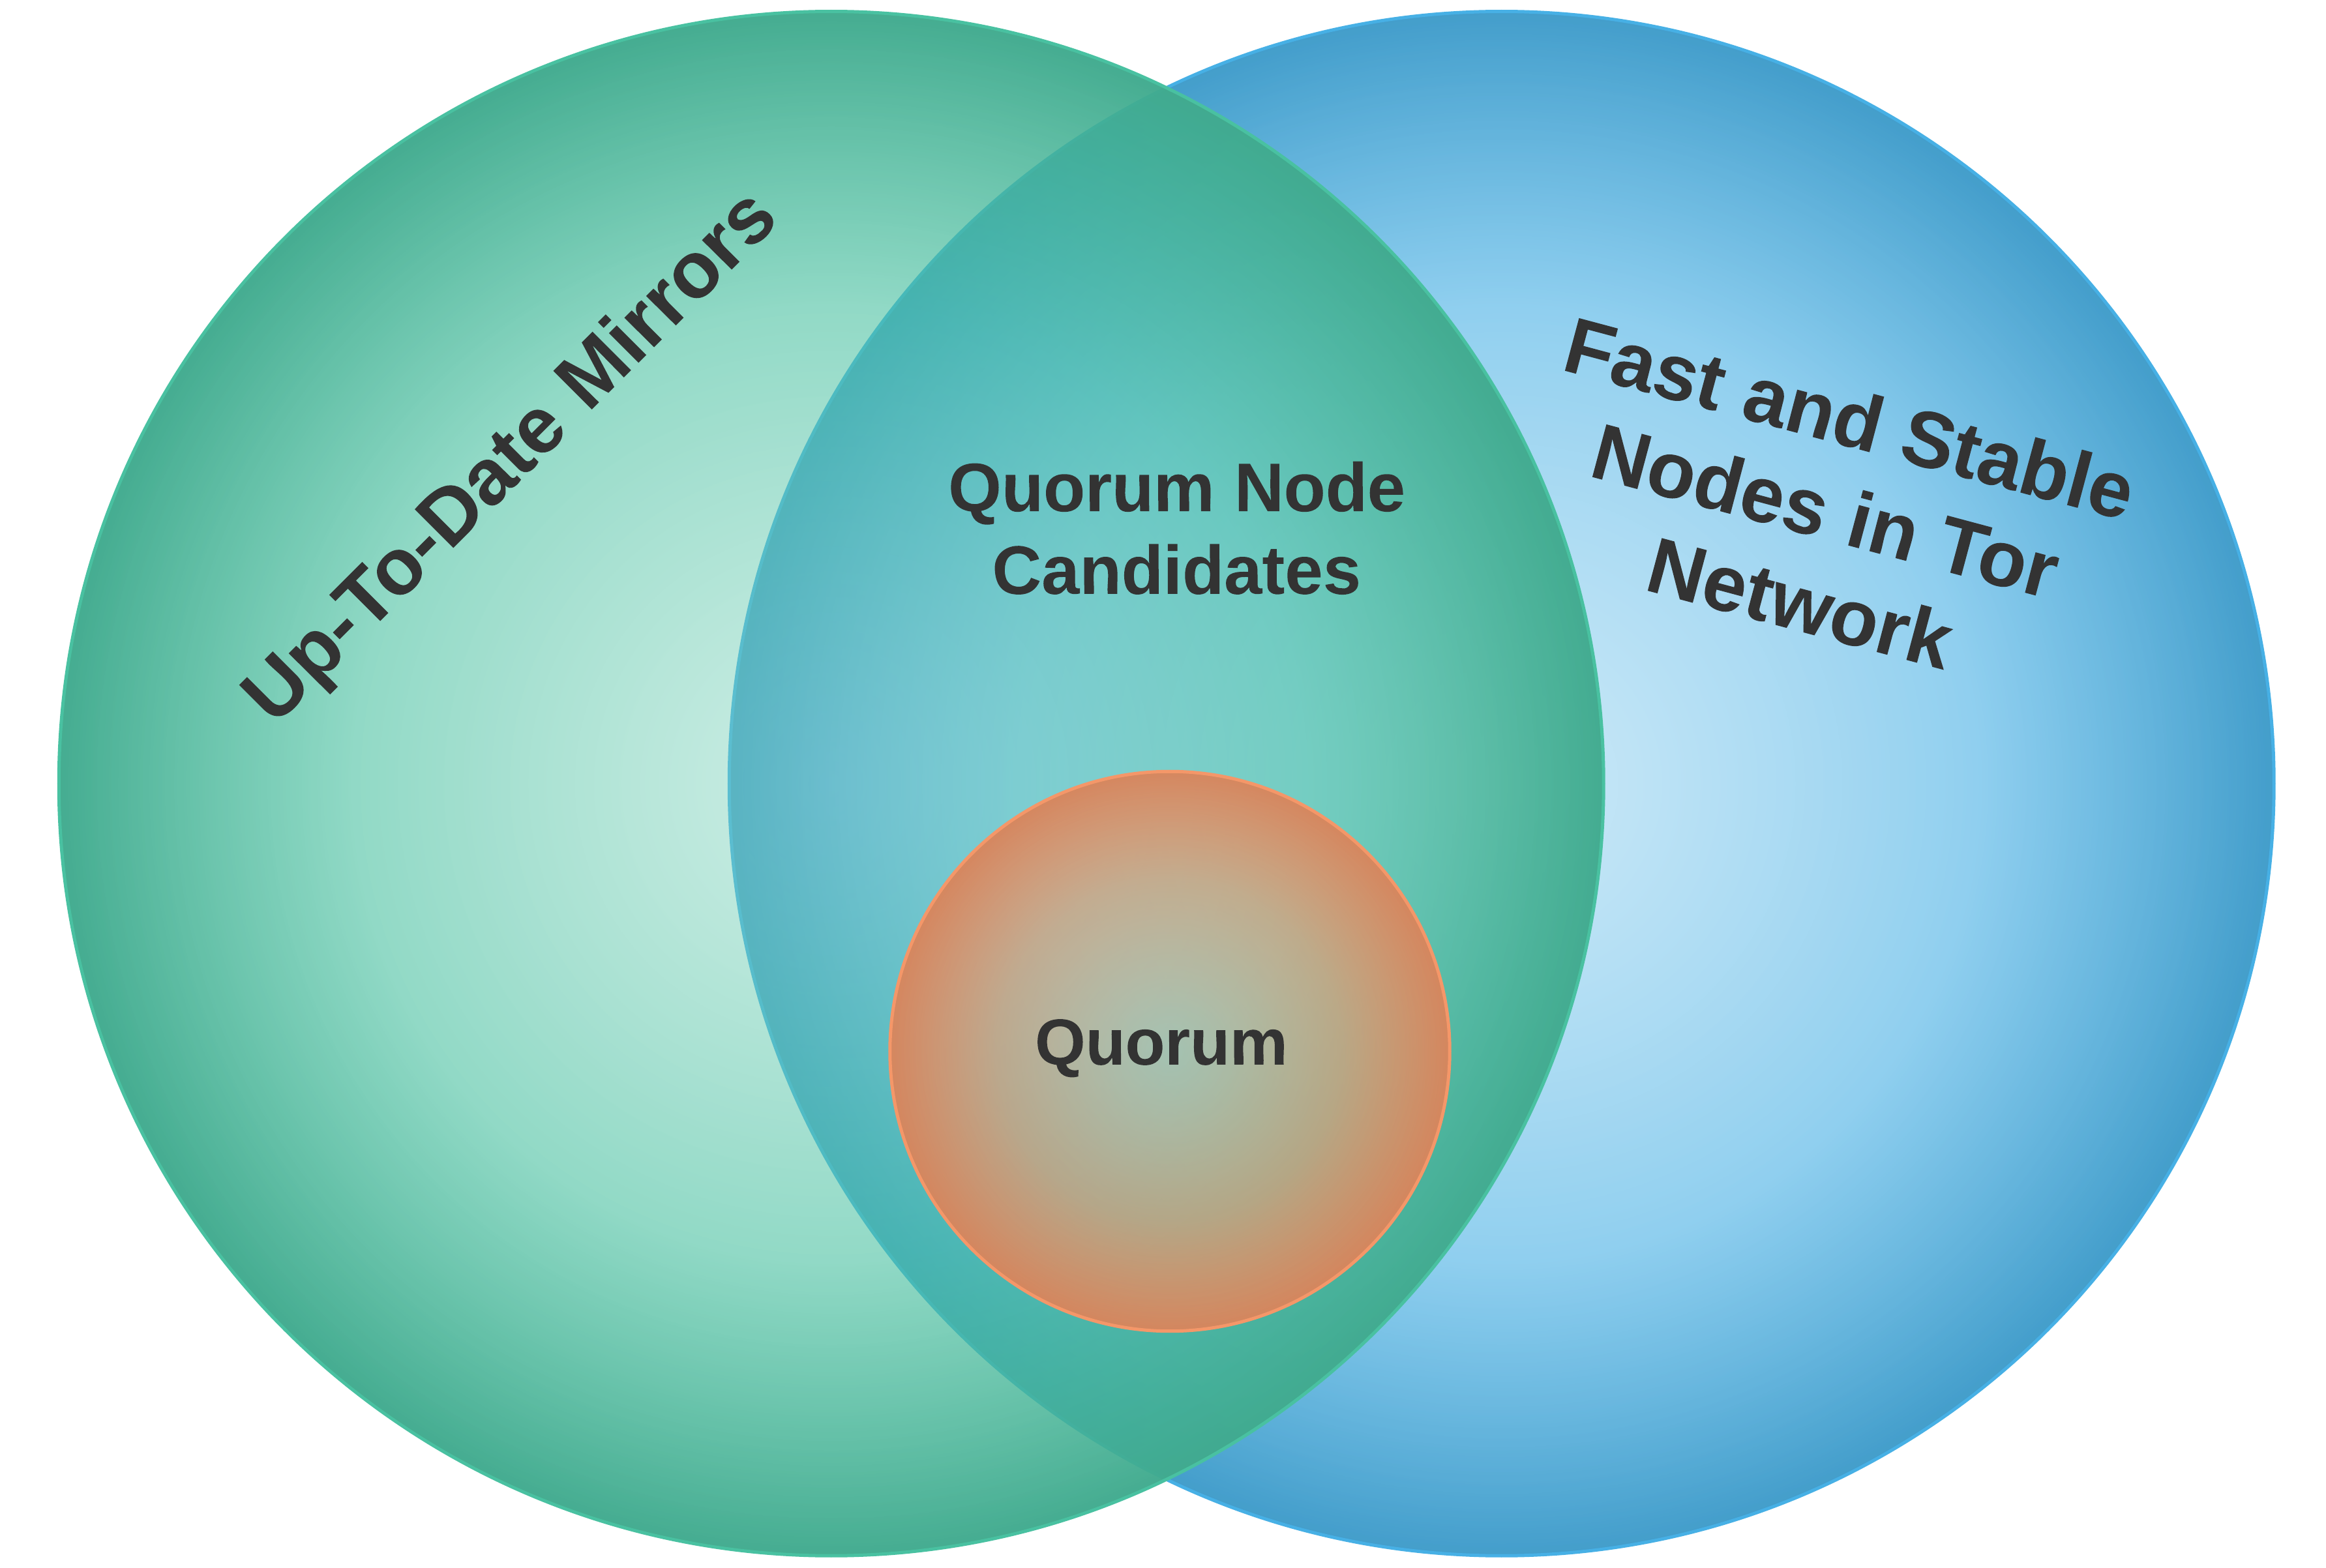
\includegraphics[width=0.5\textwidth]{images/LucidCharts/Participants.png}
	\caption{There are three sets of participants in the EsgalDNS network: \emph{mirrors}, quorum node \emph{candidates}, and \emph{quorum} members. The set of \emph{quorum} nodes is chosen from the pool of up-to-date \emph{mirrors} who are reliable nodes within the Tor network.}
\end{figure}

EsgalDNS is a distributed system and may have many participants; any machine with sufficient storage and bandwidth capacity --- including those outside the Tor network --- can obtain a full copy of all DNS information from EsgalDNS nodes. Inside the Tor network, these participants can be classified into three sets: \emph{mirrors}, quorum node \emph{candidates}, and \emph{quorum} nodes. The last set is of particular importance because \emph{quorum} nodes are the only participants to actively power EsgalDNS.

\subsection{Mirrors}

\emph{Mirrors} are Tor nodes that have performed a full synchronization (section \ref{sec:Synchronization}) against the network and hold a complete copy of all EsgalDNS data structures. This may optionally respond to passive queries from clients, but do not have power to modify any data structures. \emph{Mirrors} are the largest and simplest set of participants.

\subsection{Quorum Node Candidates}

Quorum node \emph{candidates} are \emph{mirrors} inside the Tor network that desire and qualify to become \emph{quorum} nodes. The first requirement is that they must be an up-to-date and complete \emph{mirror}, and secondly that they must have sufficient CPU and bandwidth capabilities to handle the influx of new records and the work involved with propagating these records to other \emph{mirrors}. These two requirements are essential and of equal importance for ensuring that \emph{quorum} node can accept new information and function correctly.

To meet the first requirement, Tor nodes must demonstrate their readiness to accept new records. The na\"{i}ve solution is to have Tor nodes and clients simply ask the node if it was ready, and if so, to provide proof that it's up-to-date. However, this solution quickly runs into the problem of scaling; Tor has $ \approx $ 7000 nodes and $ \approx $ 2,250,000 daily users\cite{TorMetrics}: it is infeasible for any single node to handle queries from all of them. The more practical solution is to publish information to the authority nodes that will be distributed to all parties in the consensus document. Following a full synchronization, a \emph{mirror} publishes this information in the following manner:

\begin{enumerate}
	\item Let $ tree $ be its local \emph{AVL Tree}, described in section \ref{sec:AVLTree}.
	\item Define $ s $ as SHA-384($ tree $).
	\item Encode $ s $ in Base64 and truncate to 8 bytes.
	\item Append the result to the Contact field in the relay descriptor sent to the authority nodes.
\end{enumerate}

While ideally this information could be placed in a special field set aside for this purpose, to ease integration with existing Tor infrastructure and third-party websites that parse the consensus document (such as Globe or Atlas) we use the Contact field, a user-defined optional entry that Tor relay operators typically use to list methods of contact such as email addresses and PGP keys. EsgalDNS would not be the first system to embed special information in the Contact field; onion-tip.com identifies Bitcoin addresses in the field and then sends shares of donations to that address proportional to the relay's consensus weight.

On weakness with this approach is that because this hash is published in the 00:00 GMT descriptor, an adversary could very easily forge the hash for the 01:00 GMT descriptor and onward and thus broadcast the correct hash without ever performing a synchronization. Combining this hash publication with a Time-based One-time Password Algorithm (TOTP) at a 1 hour time interval.

Of all sets of relays that publish the same hash, if \emph{mirror} $ m_{i} $ publishes a hash that is in the largest set, $ m_{i} $ meets the first qualification to become a quorum node \emph{candidate}. Relays must take care to refresh this hash whenever a new \emph{quorum} is chosen. Assuming complete honesty across all \emph{mirrors} in the Tor network, they will all publish the same hash and complete the first requirement.

The second criteria requires Tor nodes to prove that has sufficient capabilities to handle the increase in communication and processing. Fortunately, Tor's infrastructure already provides a mechanism that can be utilized to prove reliability and capacity; Tor nodes fulfil the second requirement if they have the \emph{fast}, \emph{stable}, \emph{running}, and \emph{valid} flags. These demonstrate that they have the ability to handle large amounts of traffic, have maintained a history of long uptime, are currently online, and have a correct configuration, respectively. As of February 2015, out of the ~7000 nodes participating in the Tor network, ~5400 of these node have these flags and complete the second requirement.

Both of these requirements can be determined in $ \mathcal{O}(n) $ time by anyone holding a recent or archived copy of the consensus document.

\subsection{Quorum}
\label{sec:Quorum}

\emph{Quorum} are randomly chosen from the set of quorum node \emph{candidates}. The \emph{quorum} perform the main duties of the system, namely receiving, broadcasting, and recording DNS records from hidden service operators. The \emph{quorum} can be derived from the pool of \emph{candidates} by performing by the following procedure, where $ i $ is the current day:

\begin{enumerate}
	\item Obtain a remote or local archived copy of the most recent consensus document, $ cd $, published at 00:00 GMT on day $ \floor[\big]{\frac{i}{\Delta i}} $.
	\item Extract the authorities' digital signatures, their signatures, and verify $ cd $ against $ PK_{authorities} $.
	\item Construct a numerical list, $ ql $ of quorum node \emph{candidates} from $ cd $.
	\item Initialize the Mersenne Twister PRNG with SHA-384($ cd $).
	\item Use the seeded PRNG to randomly scramble $ ql $.
	\item Let the first $ M $ nodes, numbered $ 1 .. M $, define the \emph{quorum}.
\end{enumerate}

In this manner, all parties --- in particular Tor nodes and clients --- agree on the members of the \emph{quorum} and can derive them in $ \mathcal{O}(n) $ time. As the \emph{quorum} changes every $ \Delta i $ days, \emph{quorum} nodes have an effective lifetime of $ \Delta i $ days before they are replaced by a new \emph{quorum}. Old \emph{quorum} nodes then maintain their \emph{page} (section \ref{sec:Page}) as an archive and make it available to future \emph{quorums}.

\section{Data Structures}

\subsection{Record}

A record is a simple data structure issued by hidden service operators to \emph{quorum} members. There are a number of different types of records, each representing a corresponding control operation (section \ref{sec:Operations}). However, every record includes a public hidden service key, is self-signed, and (with the exception of Delete) contains a main domain name and all subdomains under that domain name. This allows records to be referenced by their domain names as all corresponding data is encapsulated within the record itself. The details of records, their construction, their transmission, and their application in the system are described in later sections.

\subsection{Page}
\label{sec:Page}

A \emph{page} is long-term JSON-encoded textual database held by quorum nodes. It contains five fields, \emph{prevHash}, \emph{recordList}, \emph{consensusDocHash}, \emph{nodeFingerprint}, and \emph{pageSig}. 

\begin{description}
	\item[prevHash] \hfill \\
		The SHA-384 hash of \emph{prevHash}, \emph{recordList}, and \emph{consensusDocHash} of a previous page, $ p_{i - 1} $.
	\item[recordList] \hfill \\
		An array of records, sorted in a deterministic manner.
	\item[consensusDocHash] \hfill \\
		The SHA-384 of $ cd $.
	\item[nodeFingerprint] \hfill \\
		The fingerprint of the Tor node, found by generating a hash of the node's public key. This fingerprint is widely used in Tor infrastructure and in third-party tools as a unique identifier for individual Tor nodes.
	\item[pageSig] \hfill \\
		The digital signature, signed with the node's private key, of the preceding fields.
\end{description}

Each \emph{quorum} node has its own \emph{page}. If the nodes in $ quorum_{i - 1} $ remain online and our assumption the majority are acting honestly, there will exist sets (``clusters'') of \emph{pages} that have matching \emph{prevHash}, \emph{recordList}, and \emph{consensusDocHash} fields. Let the choice of $ p_{i - 1} $ in $ p_{i} $ be the most recent \emph{page} in the chain chosen by the nodes in the largest such cluster. In the event that $ p_{i - 1} $ or its records to not follow specifications described herein, $ p_{i - 1} $ should be chosen from the second largest cluster, and so on until $ p_{i - 1} $ is chosen from the largest cluster that provides a valid \emph{page}.

When a quorum node \emph{candidate} $ c_{j} $ becomes a member of the \emph{quorum}, it constructs an empty \emph{page}. If $ i = 0 $ then $ c_{j} $ sets \emph{prevHash} to zeros and generates \emph{nodeFingerprint} and \emph{pageSig}. Otherwise then $ i > 0 $ so \emph{prevHash} is set as the SHA-384 of \emph{prevHash}, \emph{recordList}, and \emph{consensusDocHash} of $ p_{i - 1} $. \emph{recordList} is set as an empty array, and \emph{consensusDocHash} and \emph{nodeFingerprint} are both defined. $ c_{j} $ then signs the preceding fields with its private key, saving the result in \emph{pageSig}. Finally, it constructs a one-hop bidirectional Tor circuit to all other \emph{quorum} nodes. These circuits are used for synchronization and must remain alive for the duration of that \emph{quorum}. Overall this creates $ \frac{M * (M - 1)}{2} $ new TCP/IP links among \emph{quorum} members.

\begin{figure}[htbp]
	\centering
	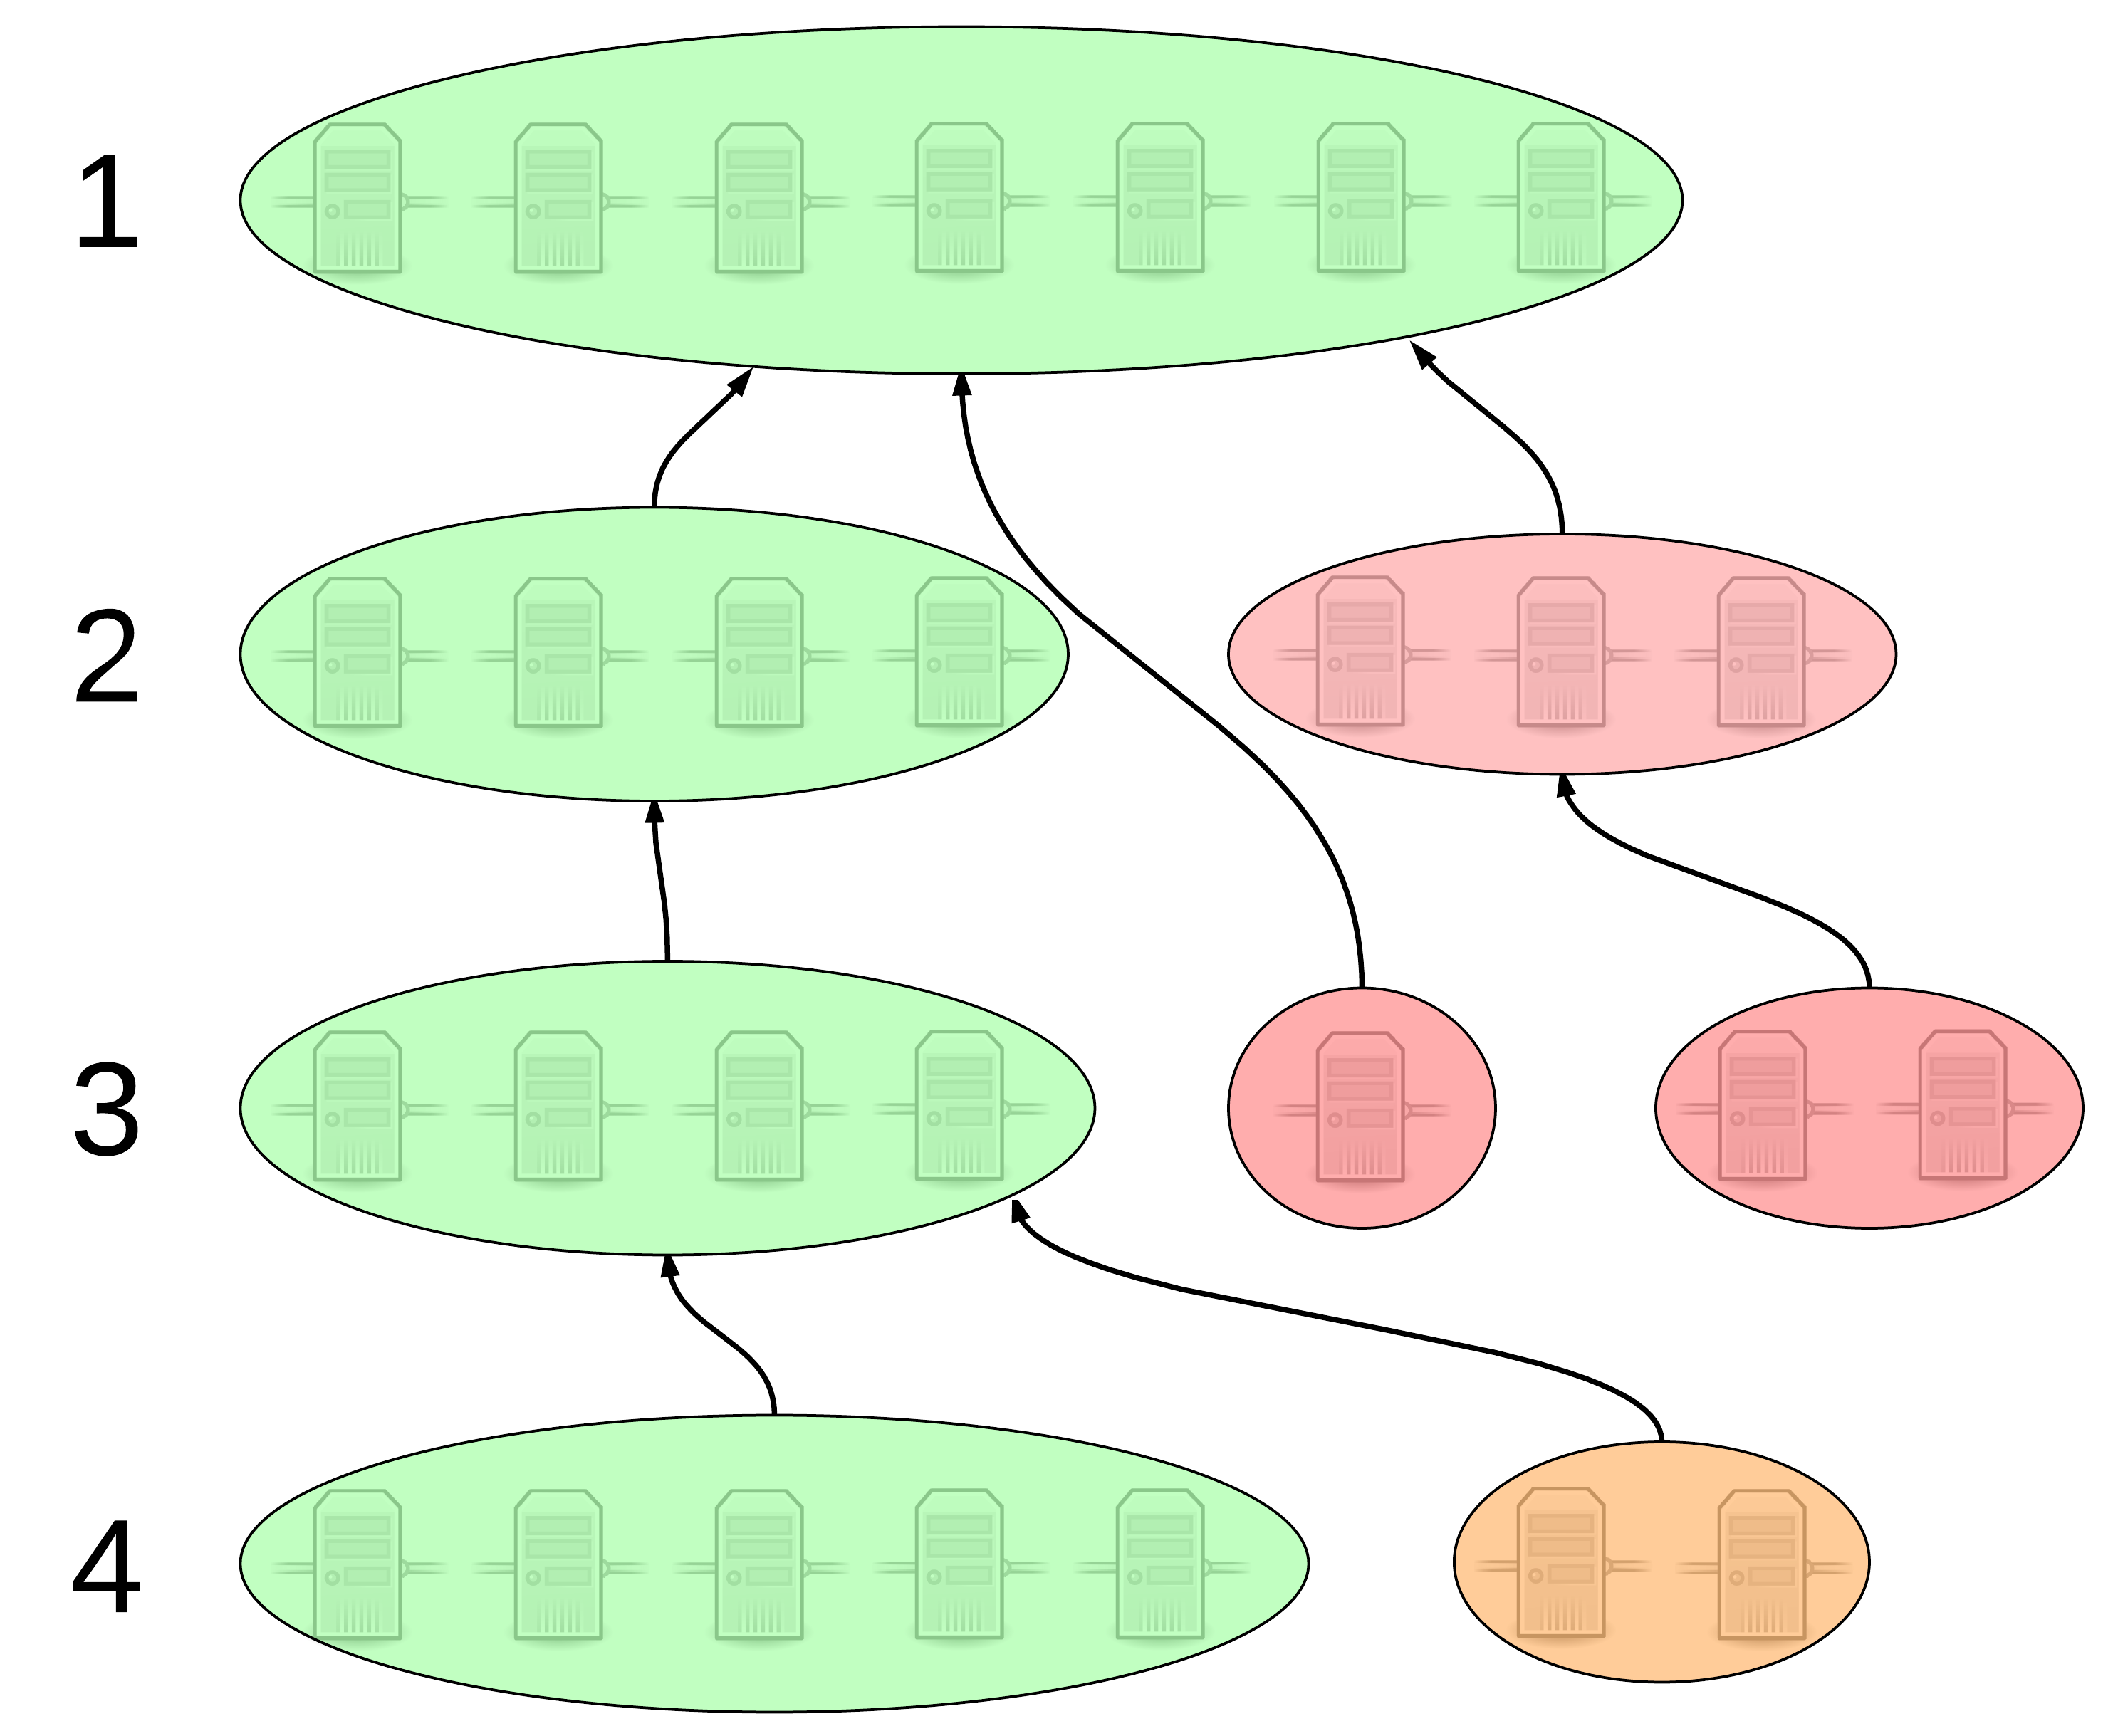
\includegraphics[width=0.7\textwidth]{images/LucidCharts/Page-chain.png}
	\caption{An example \emph{page}-chain across four \emph{quorums}. Each \emph{page} contains a references to a previous \emph{page}, forming an distributed scrolling data structure. \emph{Quorums} 1 is semi-honest and maintains its uptime, and thus has identical \emph{pages}. \emph{Quorum} 2's largest cluster is likewise in agreement, but there are three nodes which are acting maliciously together and have changed their \emph{pages}. Node 5 in \emph{quorum} 3 references an old page in attempt to bypass \emph{quorum} 2's records, and nodes 6-7 are colluding with nodes 5-7 from \emph{quorum} 2. Finally, \emph{quorum} 3 has two nodes that acted honestly but did not record new records, so their \emph{page}-chains differ from the others. However, across all four days the largest clusters are honest nodes and thus integrity remains in the \emph{page}-chain.}
\end{figure}


%Each \emph{quorum} node holds its page, the pages of the other quorum nodes on that day, and a single archive of the consensus document. 


\subsection{Snapshot}

Similar to a page, a \emph{snapshot} is JSON-encoded textual database held by \emph{quorum} nodes, but unlike pages, \emph{snapshots} are short-term and volatile. They are used for propagating very new records and receiving records from other active \emph{quorum} nodes. Snapshots contain three fields: \emph{originTime}, \emph{recentRecords}, \emph{nodeFingerprint}, and \emph{snapshotSig}.

\begin{description}
	\item[originTime] \hfill \\
		Unix time when the snapshot was first created.
	\item[recentRecords] \hfill \\
		A list of records.
	\item[nodeFingerprint] \hfill \\
		The fingerprint of the Tor node.
	\item[snapshotSig] \hfill \\
		The digital signature of the preceding fields, signed using the node's private key.
\end{description}

\emph{Snapshots} are generated every $ \Delta s $ minutes. At the beginning of one of these intervals, a \emph{quorum} node generates an empty \emph{snapshot}. \emph{OriginTime} is set to the current Unix time, \emph{recentRecords} is an empty array, \emph{nodeFingerprint} is set the same as it is for a \emph{page}, and \emph{snapshotSig} is generated. As records are received, a \emph{quorum} node merges the record into their \emph{snapshot}, as described in section \ref{sec:Broadcast}.

\subsection{AVL Tree}
\label{sec:AVLTree}

A self-balancing binary AVL tree is used as a local cache of existing records. Its nodes hold references to the location of records in a local copy of the \emph{page}-chain, and it is sorted by alphabetical comparison of domain names. As a \emph{page}-chain is a linear data structure that requires a $ \mathcal{O}(n) $ scan to find a record, the $ \mathcal{O}(n\log{}n) $ generation of an AVL tree cache allows lookups of domain names to occur in $ \mathcal{O}(\log{}n) $ time. An AVL tree is generated from a \emph{page}-chain, as described in section \ref{sec:Synchronization}.

% todo: illustration of an AVL tree with pointers to page-chain records


% this really could be a Merkle tree, then the top root could be published in the consensus doc

% todo: this works well for names, but how about for Moves?
% records that are less than a day old will have a hard time with the hashtable, but once in a page they are good

\subsection{Hashtable Bitset}

%  and claim that a domain name does not exist when in fact it does

% at startup, clients should be given the root of the Merkle tree for the hashtable collisions, or at least hashes in the tree

A hashtable bitset is a special and highly compact adaptation of a traditional hashtable. Unlike its AVL tree counterpart, the purpose of the hashtable bitset is to prove the non-existence of a record. Demonstrating non-existence is a challenge often overlooked in DNS: even if the DNS records can be authenticated by a recipient, (i.e. an SSL certificate or EsgalDNS self-signed records) a DNS resolver may lie to a client and claim a false negative on the existence of a domain name. Aside from trusting the response of a central authority or a local DNS server, a client cannot easily determine the accuracy of this response without downloading all the records and checking for themselves, but this is impractical in most environments. Asking a central trusted authority or a group of authorities (e.g. the \emph{quorum}) for verification is a simple solution, but these queries introduce additional load upon the authorities. The hashtable bitset allows a set of trusted authorities to publish a digitally signed data structure that allows local resolvers to prove non-existence for any non-existent domain name in $ \mathcal{O}(1) $ time on average, and with minimal data sent to the client. We extend the data structure by resolving collisions in a manner that eliminates false negatives and allows the proof of non-existence claims in $ \mathcal{O}(\log{}n) $ in the worst case.

Like an ordinary hashtable, the hashtable bitset maps keys to buckets, but in this application it is only necessary to track the existence of a domain name. Therefore we represent each bucket as a bit, creating a compact bitset of $ C * n $ size, where $ n $ is the number of existing domain names and $ c $ is some constant coefficient. The hashtable bitset records a ``1'' if a domain name exists, and a ``0'' if not. In the event of a hash collision, all records that map to that bucket should be added to an array list. Following the construction of the bitset, the array should be sorted alphabetically by domain name and then converted into a Merkle tree. A client can verify non-existence by confirming that the hash of the requested domain name points to a 0, or if it points to a 1 and the DNS resolver claims non-existence, the resolver must demonstrate it by sending the client the appropriate section of the Merkle tree, as described in section \ref{sec:DomainQuery}.

Trusted authorities (e.g. the \emph{quorum} of size $ M $) can divide the bitset into $ Q $ sections, digitally sign each section, and digitally sign the root hash of the Merkle tree. This allows a DNS resolver to send a $ \frac{C * n}{Q} $-sized section of the bitset and its digital signatures to the client, rather than sending the entire bitmap, which may be larger than $ \frac{C * n}{Q} $ for some choices of $ C $, $ Q $, and the size of the signatures. The assembly of these signatures is detailed in \ref{sec:Broadcast}.

Note that a Bloom filter with $ k $ hash functions could be used instead of a compact hashtable, but a Bloom filter would require sending up to $ k $ sections of buckets to the client. Therefore, we use a simple hashtable scheme, which is effectively a Bloom filter with $ k = 1 $.

% Additionally, after signing, the Bloom filter would require $ \mathcal{O}(C * n * k * Q * M) $ space, rather than $ \mathcal{O}(C * n * Q * M) $

% merkle tree: leafs contain <domain name, recordHash>?

% since we already have in this application it is only necessary to track whether a domain name exists or not. Therefore we represent each bucket as a bit. 

\section{Operations}
\label{sec:Operations}

\subsection{Synchronization}
\label{sec:Synchronization}

EsgalDNS records are public knowledge and any machine may download a complete copy of all data structures that encapsulate records. Once the synchronization is complete, that machine becomes a \emph{mirror} and can be a server to other machines, like BitTorrent or other peer-to-peer networks.

Let $ i $ be the current day, $ \Delta i $ be the lifetime of the \emph{quorum}, Alice be the machine becoming a \emph{mirror}, and Bob an existing \emph{mirror}. 

\begin{enumerate}
	\item Alice obtains from Bob his $ \min(i,L) $ most recent \emph{pages} in his cached \emph{page}-chain, where $ L $ is the lifetime of records.
	\item Alice also obtains the SHA-384 hash, $ h_{p} $, of the concatenation of \emph{prevHash}, \emph{recordList}, and \emph{consensusDocHash} for the \emph{page} used by each \emph{quorum} node for all \emph{quorums} between $ i - \min(i,L) $ and $ i $. Note that each $ h_{p} $ is digitally signed by its respective \emph{quorum} node. See section \ref{sec:Broadcast} for details on how this information is available to Bob.
	\item Alice downloads the $ \frac{\min(i,L)}{\Delta i} $ consensus documents published every $ \Delta i $ days at 00:00 GMT between days $ i - \min(i,L) $ and $ i $. Alice may download these documents from Bob, but to lighten the burden on Bob she may also obtain them from any other source. Bob may have compressed these beforehand to save space: very high compression ratios can be achieved under 7zip.
	\item The last item that Alice fetches from Bob is the hashtable bitset and the root of the Merkle collision table, which has been signed by all current \emph{quorum} members.
	\item Starting with the oldest available consensus document and working forward to day $ \floor[\big]{\frac{i}{\Delta i}} $, 
		\begin{enumerate}
			\item Alice follows the procedures described in section \ref{sec:Quorum} to calculate the old \emph{quorum}.
			\item She confirms that the oldest \emph{page} she received from Bob is held by the largest cluster of agreeing \emph{quorum} nodes.
			\item Alice verifies the validity of the \emph{page} and the records contained within it.
			\item Finally, Alice progresses to the next most recent \emph{page}, repeating the procedure but also verifying that the \emph{prevHash} refers the $ p_{i - 1} $ she was just examining. This process repeats until all $ \min(i,L) $ \emph{pages} have been verified.
		\end{enumerate}
	\item Alice extracts all records from the now-validated \emph{page}-chain and constructs the AVL tree and the hashtable bitset with its Merkle tree containing the collisions. As domains expire every $ L $ rotations of the \emph{quorum}, recent Create, Modify, Move, and Renew operations all act as renewals of the domain name and thus are used by Alice to generated these structures. She should process the records in reverse chronological order because a Delete operation causes immediate expiration of an existing domain.
	\item She confirms that the signatures on the sections of the bitset and the signatures on the Merkle root hash check out against her generated copy. If they do not, Bob may have manipulated the data and she may need to ask someone else.
	\item Finally, Alice may make the \emph{page}-chain and consensus documents that she downloaded from Bob and the binary hashtable that she constructed available to others. She may also respond to Domain and Onion Queries using the AVL tree. She must perform these actions once Alice becomes a quorum member \emph{candidate}.
\end{enumerate}

\subsection{Broadcast}
\label{sec:Broadcast}

% cite paper that shows why recycling the entry node is a good idea
% possible that a malicious node could see his transmission, ignore it, then claim it themselves

Operation records, such as Create, Modify, Move, Renew, and Delete must anonymously transmitted through a Tor circuit to the \emph{quorum} by a hidden service operator. First, the operator uses a Tor circuit to fetch from a \emph{mirror} the consensus document on day $ \floor[\big]{\frac{i}{\Delta i}} $ at 00:00 GMT, which he then uses to derive the current \emph{quorum}. Secondly, he asks the \emph{mirror} for the digitally signed hash of the \emph{page} used by each \emph{quorum} node. Third, he randomly selects two \emph{quorum} nodes from the largest cluster of matching \emph{pages} and sends his record to one of them. For security purposes, the operator should use the same entry node for this transmission that their hidden service uses for its communication. The \emph{quorum} node may reject his record if it is invalid, otherwise it accepts it. Fourth, he constructs a circuit to the second node and polls the node 15 minutes later to determine if it has knowledge of the record. If it does, he can be reasonable sure that the record has been properly transmitted and recorded. If the record is not known the next day, the operator should repeat this procedure to ensure that the record is recorded in the \emph{page}-chain.

Each \emph{quorum} node buffers received records into a \emph{snapshot} and then flushing the snapshot to the rest of the \emph{quorum} every $ T $ minutes by performing the following :

Let $ x $ be the current propagation iteration and $ snap_{x} $ be the currently-active snapshot filled with records over the last $ T $ minutes.

\begin{enumerate}
	\item Generates a new snapshot, labelled $ snap_{x+1} $, sets \emph{originTime} to the current time, creates \emph{snapshotSig}, and sets $ snap_{x+1} $ to be the currently active snapshot for collecting new records.
	\item Define an empty array list $ arr $.
	\item With each node $ q_{k \ne j} $ in the \emph{quorum} using its existing one-hop Tor circuits, 
		\begin{enumerate}
			\item Sends its $ snap_{x} $ and $ <pageSig_{q_{j}}, nodeFingerprint_{q_{j}}> $, every $ <pageSig_{q_{k}}, nodeFingerprint_{q_{k}}> $ it has received so far, and its signatures on the sections of the hashtable bitset and on the Merkle tree root to $ q_{k} $.
			\item Receives $ s_{x, k} $ and $ <pageSig_{q_{k}}, nodeFingerprint_{q_{k}}> $ from $ q_{k} $.
			\item Archives $ <pageSig_{q_{k}}, nodeFingerprint_{q_{k}}> $ and add any records that did not exist in $ snap_{x} $ to $ arr $.
		\end{enumerate}
	\item For any missing $ <pageSig_{q_{k}}, nodeFingerprint_{q_{k}}> $, it asks a random \emph{quorum} member $ q_{i \ne k} $ for $ q_{k} $'s $ pageSig_{q_{k}} $. In this way, it has a list of \emph{page} signatures from all \emph{quorum} nodes.
	\item Merges $ snap_{x} $ and the records in $ arr $ into its \emph{page} and regenerates \emph{pageSig}.
	\item Updates its AVL tree, hashtable bitset, and Merkle collision tree, and regenerates the signatures on the bitset and on the Merkle root tree.
	\item Increments $ x $.
\end{enumerate}

This process is illustrated in figure \ref{fig:recordBroadcast}.

\begin{figure}[htbp]
	\centering
	\begin{tikzpicture}[->, node distance=2.5cm, main node/.style={circle, fill=blue!20, draw, font=\sffamily\Large\bfseries}]

			\node[main node] (1) {$ Q_{1} $};
			\node[main node] (2) [right of=1] {$ Q_{2} $};
			\node[main node] (3) [right of=2] {};
			\node[main node] (4) [right of=3] {$ Q_{3} $};

			\node[main node] (5) [below of=1] {};
			\node[main node] (6) [right of=5] {$ Q_{4} $};
			\node[main node] (7) [right of=6] {};
			\node[main node] (8) [right of=7] {};
		  
			\node[main node, font=\small] (9) [below of=5] {$ N_{middle} $};
			\node[main node] (10) [right of=9] {};
			\node[main node, font=\small] (11) [right of=10] {$ N_{ip} $};
			\node[main node] (12) [right of=11] {$ Q_{5} $};

			\node[main node] (13) [below of=9] {};
			\node[main node] (14) [right of=13] {};
			\node[main node, font=\small] (15) [right of=14] {$ N_{entry} $};
			\node[main node] (16) [right of=15] {HS};
			
			% draw 1st and 2nd part of circuit
			\tikzstyle{EdgeStyle}=[bend right=12, -, green]
			\Edge[](16)(15)
			\Edge[](9)(15)
			
			% draw last part of circuit
			\tikzstyle{EdgeStyle}=[bend left=17, -, green]
			\Edge[](9)(11)
			
			% draw record moving from exit to 1st q. node
			\draw[thick, red, <-, postaction={decorate, decoration={text along path, text align=center, text={record}, raise=3pt}}] (6) to [bend right=15] (11){};
			
			% draw upper left propegation
			\tikzstyle{EdgeStyle}=[bend left=12, ->, blue]
			\Edge[](6)(2)
			\Edge[](6)(1)
			
			% draw upper right propegation
			\tikzstyle{EdgeStyle}=[bend left=20, ->, blue]
			\Edge[](6)(12)
			\draw[thick, blue, postaction={decorate, decoration={text along path, text align=center, text={snapshot}, raise=3pt}}] (6) to [bend right=18] (4){};

		\end{tikzpicture}
	\caption{The hidden service operator uses his existing circuit (green) to inform \emph{quorum} node $ Q_{4} $ of the new record. $ Q_{4} $ then distributes it via \emph{snapshots} to all other \emph{quorum} nodes. Each records it in their own \emph{page} for long-term storage.}
	\label{fig:recordBroadcast}
\end{figure}

\subsection{Create}

Any hidden service operator may claim any domain name that is not currently in use. As domain names cannot be purchased from a central authority, it is necessary to implement a system that introduces a cost of ownership. This performs three main purposes: 

\begin{enumerate}
	\item Thwarts potential flooding of the system with domain registrations.
	\item Introduces a cost of investment that encourages the availability of hidden services.
	\item Makes domain squatting more difficulty, where someone claims one or more domains on a whim for the sole purpose of denying them to others. As hidden service operators typically remain anonymous, it is difficulty for one to contact them and request relinquishing of a domain, nor is there a central authority to force relinquishing through a court order or other formal means.
\end{enumerate}

Therefore we incorporate a proof-of-work scheme that makes registration computationally intensive but is also easily verified by anyone. A Create record consists of nine components: \emph{type}, \emph{nameList}, \emph{contact}, \emph{timestamp}, \emph{consensusHash}, \emph{nonce}, \emph{pow}, \emph{recordSig}, and \emph{pubHSKey}. Let the variable \emph{central} consist of all fields except \emph{recordSig} and \emph{pow}. Fields that are optional are blank unless specified, and all fields are encoded in base64, except for \emph{nameList}, \emph{contact}, and \emph{timestamp}, which are encoded in standard UTF-8.

\begin{center}
    \begin{tabular}{ | l | l | p{9cm} |}
    \hline
    \textbf{Field} & \textbf{Required?} & \textbf{Description} \\ \hline
    type & Yes & A textual label containing the type of record. In this case, \emph{type} is set to ``Create''. \\ \hline
    nameList & Yes & An array list of up to 24 domain names. Here a domain name consists of one or more textual labels that are delimited by dots. Domain names use the .tor TLD. There can be up to eight name-separator pairs prefixing the .tor postfix, and each name can be up to 32 characters long. These must have a base domain name listed in this field so that hidden service operators cannot claim subdomains on a base domain name that they do not own. However, domain names can point to domains with either .tor or .onion TLDs. \\ \hline
    contact & No & The fingerprint of the HS operator's PGP key, if he has one. If the fingerprint is listed, clients may query a public keyserver for this fingerprint, obtain the operator's PGP public key, and contact him over encrypted email. \\ \hline
	timestamp & Yes & The UNIX timestamp of when the operator created the registration and began the proof-of-work to validate it. \\ \hline
	consensusHash & Yes & The SHA-384 hash of the morning's consensus document at the time of registration. This is a provable timestamp, since it can be matched against archives of the consensus document. Quorum nodes will not accept registration records that reference a consensus document more than 48 hours old. \\ \hline
	nonce & Yes & Four bytes that serve as a source of randomness for the proof-of-work, described below. \\ \hline
    pow & Yes & 16 bytes that demonstrate the result of the proof-of-work. \\ \hline
    recordSig & Yes & The digital signature of all preceding fields, signed using the hidden service's private key. \\ \hline
    pubHSKey & Yes & The public key of the hidden service. If the operator is claiming a subdomain of any depth, this key must match the \emph{pubHSKey} of the top domain name.\\ \hline
    \end{tabular}
\end{center}

A record is made valid through the completion of the proof-of-work process. The hidden service operator must find a \emph{nonce} such that the SHA-384 of \emph{central}, \emph{pow}, and \emph{recordSig} is $ \leq 2^\textrm{difficulty} $, where \emph{difficulty} specifies the order of magnitude of the work that must be done. The \emph{difficulty} is doubled every 1460 days. For each \emph{nonce}, \emph{pow} and \emph{recordSig} must be regenerated, which effectively forces the computation to be performed by a machine owned by the HS operator. When the proof-of-work is complete, the valid and complete record is represented in JSON format for transmission to the \emph{quorum}.

%\emph{TODO: specify how difficulty increases to counteract Moore's Law. Also, is the pow even necessary, or can that be regenerated by anyone?}

% "domain name" is used throughout when not talking about example.tor, it's used generically.

\subsection{Modify}

If a hidden service operator wishes to update his registration with more current information, he can broadcast a Modify record. The Modify record has identical fields to Create, but \emph{type} is set to ``Modify''. The operator creates a Modify record with the corrected information and then sends it to the \emph{quorum}. The Modify operation renews the ownership of single-label domain names, so a record of the domain name must already exist in the \emph{page}-chain and be less than $ L $ days old. Once received, \emph{quorum} nodes update the leaf in their AVL trees with the modified record. Modify records have a difficulty of $ \frac{\textrm{difficulty}_{Create}}{4} $.

\subsection{Move}

%todo: this is trickier and needs more thought

A Move record may be issued if a hidden service operator wishes to transfer domain names in a record to another owner. Move records have all the fields of a Create record, have their \emph{type} is set to ``Move'', and contain one additional field: the public key of the new owner. Like Modify records, Move records also renew single-label domain names, so they must already exist in the \emph{page}-chain. Move records also have a difficulty of $ \frac{\textrm{difficulty}_{Create}}{4} $.

% A hidden service operator may transfer one or more domains to a new owner. The transfer record contains the public key and signature of the originating owner and the public key of the new owner. Subdomains that are not explicitly moved to the new owner are invalid and can be reclaimed by the new owner if they wish. The proof-of-work cost is an eighth of domain registration.

\subsection{Renew}

As single-label domain names expire every $ L $ days because records older than $ L $ are not fetched by \emph{mirrors}, Renew records must be reissued periodically to ensure that the domain names remain in the \emph{page}-chain. Renew records are identical to Create records, except that \emph{type} is set to ``Renew'' and, like the Modify and Move records, the difficulty is $ \frac{\textrm{difficulty}_{Create}}{4} $.

%Subdomains, as they must match the ownership of the top domain, have no expiration themselves but rather will expire when the domain does.

\subsection{Delete}

Delete records are useful if a hidden service operator wishes to relinquish ownership rights over domain names, or if they consider their private key compromised. Delete records are also identical to Create records, but they have \emph{type} is set to ``Delete'' and any single-label domain names and subdomains are instantly purged from the caches in all \emph{mirror} nodes and thus become available to others. There is no difficutly cost associated with Delete records, so they can be issued instantly.

\subsection{Domain Query}
\label{sec:DomainQuery}

% todo: recursive resolution of the name, check for deleted or moved domains

% queries: first check the hashtable, then check the AVL tree

When a Tor user Alice wishes to visit example.tor, her client software must perform a query to obtain the .onion address that corresponds to that domain name. To meet our original requirements, Alice must be able to verify that the received record originated from the desired hidden service (akin to SSL certificates on the Clearnet), the lookup must happen in a privacy-enhanced manner, and the details of the query must be handled behind-the-scenes, invisibly to the user.

At startup, Alice builds a circuit to any \emph{candidate} node $ n_{s} $ that meets the qualification requirements previously described. Alice then asks $ n_{s} $ for the desired name and a verification level, which is 0 if not specified. As we mentioned in the Requirements section, it is impractical to require Alice to perform a full synchronization and download all \emph{pages} in order to verify the uniqueness and trustworthiness of a returned record. Therefore Alice can rely on her existing at least partial trust of the Tor network and perform various degrees of verification with minimal information.

If Alice's verification level is 0, $ n_{s} $ returns only the Registration record or the Ownership Transfer record, whichever is newer. Alice extracts the fields, uses \emph{pubHSKey} to confirm that \emph{recordSig} verifies the record, then confirms the proof-of-work. Finally, Alice uses \emph{pubHSKey} to generate the hidden service .onion address (16 bytes of the base58-encoded SHA-1 hash of \emph{pubHSKey} in PKCS.1 DER encoding) and looks up the hidden service in the traditional manner. The lookup fails if the service has not published a recent hidden service desciptor to the distributed hash table, otherwise the lookup goes through. End-to-end verification is complete when \emph{pubHSKey} can be successfully used to encrypt the hidden service cookie and the service proves that it can decrypt $ sec $.

If Alice requests verification level 1, $ n_{s} $ returns the record, a \emph{page} from any \emph{quorum} node that contained it, and and an archive of the consensus document. Alice can verify the authenticity of the consensus document, can determine the \emph{quorum} and extract their keys, and verify the \emph{page} that $ n_{s} $ gave her. Alice then proceeds with record verification and hidden service lookup, as specified in level 1.

At level 2, $ n_{s} $ returns to Alice all material from level 1, but also includes \emph{pageSig} from all \emph{quorum} nodes on that day. This is width verification as Alice can confirm that the majority of the \emph{quorum} used that \emph{page}, and that $ n_{s} $ didn't pick a \emph{quorum} node that performed abnormally.

At level 3, $ n_{s} $ returns the same as level 1, but also sends the \emph{pages} that form the chain below it. Alice can confirm this depth verification by following the \emph{page}-chain back in time, obtaining the old consensus documents, and verifying the \emph{pageSigs} and the records contained within every \emph{page}. This is a very thorough level of verification but is also very demanding in terms of computation and bandwidth usage.

As an optimization, $ n_{s} $ may have queried Tor's distributed hash table for the hidden service in advance and cached its introduction point. $ n_{s} $ can then return to Alice this introduction point, significantly improving performance on Alice's end because she would not need to query the hash table herself and can simply skip to building circuits to the hidden service.

%The scroll is a distributed and highly redundant chained data structure that slowly rolls through the Tor network. The scroll is $ N $ by $ M $ in shape and consists of two primary components: \emph{blocks} and \emph{captures}. Blocks contain one or more captures, and blocks are duplicated across the $ M $ committee nodes. Each capture is a collection of information from one day; it contains the consensus document from the previous morning, a list of domain registrations approved that day, the approval sign-off digital signatures from the committee nodes on those registrations, the digital signatures from the committee indicating their approval of the integrity of the scroll, and the hash of the previous four captures. In this way, captures are fully verifiable and contain enough information to link to the previous capture, forming a chain. This chain is not held by any single Tor node, rather it is encapsulated within a rolling window of blocks $ N $ days deep. As the days progress, the captures in the oldest block are migrated to the current day's block, rolling the structure forward. Thus the scroll is divided across $ N $ blocks, with copies of each block held by $ M $ Tor nodes. I consider $ N = 16, M = 64 $ reasonable values, which would involve 1,024 nodes at any given time, although $ M $ can be easily changed even while the scroll is in use.

\subsection{Onion Query}

\section{Examples and Structural Induction}

\subsection{Base Case}

In the most trivial base case of a single quorum node \emph{candidate} $ c_{1} $, a hidden service Bob, and a Tor client Alice, the procedures are relatively simple. On $ \textrm{day}_{0} $, $ c_{1} $ generates an initial page $ p_{1,1} $ containing no records and signs $ p_{1,1} $, but does not accept records for this initial page. $ p_{1,1} $ appears in Figure \ref{fig:emptyPage}.

\begin{figure}
	\begin{lstlisting}
	{
		"prevHash": 0,
		"recordList": [],
		"consensusDocHash": "uU0nuZNNPgilLlLX2n2r+sSE7+N6U4DukIj3rOLvzek=",
		"nodeFingerprint": "2FC06226AE152FBAB7620BB107CDEF0E70876A7B",
		"pageSig": "KSaOfzrXIZclHFcYxI+3jBwLs943wxVv3npI5ccY/kBEpyXRSopzjoFs746n0tJqUpdY4Kbe6DBwERaN7ELmSSK9Pu6q8QeKzNAh+QOnKl0fKBN7fqowjkQ3ktFkR0Vuox9WrrbNTMa4+up0Np52hlbKA3zSRz4fbR9NVlh6uuQ="
	}
	\end{lstlisting}
	\caption{A sample empty \emph{page}, $ p_{1,1} $, encoded in JSON and base64.}
	\label{fig:emptyPage}
\end{figure}

On $ \textrm{day}_{1} $, $ c_{1} $ examines its database of page-chains and generates a new page, $ p_{2,1} $, that references $ p_{1,1} $, a chain with 0 references, the most in the database. The hidden service \emph{Bob} hashes the consensus document, generating \emph{T/q7q052MgJGLfH1mBGUQSF YjwVn9VvOWBoOmevPZgY=} which is then fed into the Mersenne Twister to scramble the list of \emph{candidate} nodes. Since $ c_{1} $ is the only \emph{candidate}, he is chosen a member of the \emph{quorum}. Bob then builds a circuit to $ c_{1} $, and sends him a registration record, $ r_{reg} $, which appears in Figure \ref{fig:sampleRecord}. 

\begin{figure}
	\begin{lstlisting}
	{
		"names": {
			"example.tor": "exampleruyw6wgve.onion",
			"sub.example.tor": "example.tor"
		}
		"contact": "AD97364FC20BEC80",
		"timestamp": 1424045024,
		"consensusHash": "uU0nuZNNPgilLlLX2n2r+sSE7+N6U4DukIj3rOLvzek=",
		"nonce": "AAAABw==",
		"pow": "4I4dzaBwi4AIZW8s2m0hQQ==",
		"recordSig": 	"KSaOfzrXIZclHFcYxI+3jBwLs943wxVv3npI5ccY/kBEpyXRSopzjoFs746n0tJqUpdY4Kbe6DBwERaN7ELmSSK9Pu6q8QeKzNAh+QOnKl0fKBN7fqowjkQ3ktFkR0Vuox9WrrbNTMa4+up0Np52hlbKA3zSRz4fbR9NVlh6uuQ=",
		"pubHSKey": "MIGhMA0GCSqGSIb3DQEBAQUAA4GPADCBiwKBgQDE7CP/kgwtJhTTc4JpuPkvA7Ln9wgc+fgTKgkyUp1zusxgUAn1c1MGx4YhO42KPB7dyZOf3pcRk94XsYFY1ULkF2+tf9KdNe7GFzJyMFCQENnUcVXbcwLH4vAeiGK7R/nScbCbyc9LT+VE1fbKchTL1QzLVBLqJTxhR+9YPi8x+QIFAdZ8BJs="
	}
	\end{lstlisting}
	\caption{Sample registration record from a hidden service, encoded in JSON and base64. The ``sub.example.tor'' $ \to $ ``example.tor'' $ \to $ ``exampleruyw6wgve.onion'' references can be resolved recursively.}
	\label{fig:sampleRecord}
\end{figure}

$ c_{1} $ can continue to accept and insert records in this way, but if $ r_{reg} $ is the only one that $ c_{1} $ receives, at the next 15 minute mark $ c_{1} $ will attempt to propagate this snapshot to other \emph{quorum} nodes. However, as $ c_{1} $ is the only \emph{quorum} node, that step is not necessary here. $ c_{1} $ then adds $ r_{reg} $ into its page, creating $ p_{1,1} $, shown in Figure \ref{fig:c1page}.

\begin{figure}
	\begin{lstlisting}
	{
		"prevHash": 0,
		"recordList": [
			{
				"names": {
				"example.tor": "exampleruyw6wgve.onion",
				"sub.example.tor": "example.tor"
			}
			"contact": "AD97364FC20BEC80",
			"timestamp": 1424045024,
			"consensusHash": "uU0nuZNNPgilLlLX2n2r+sSE7+N6U4DukIj3rOLvzek=",
			"nonce": "AAAABw==",
			"pow": "4I4dzaBwi4AIZW8s2m0hQQ==",
			"recordSig": 	"KSaOfzrXIZclHFcYxI+3jBwLs943wxVv3npI5ccY/kBEpyXRSopzjoFs746n0tJqUpdY4Kbe6DBwERaN7ELmSSK9Pu6q8QeKzNAh+QOnKl0fKBN7fqowjkQ3ktFkR0Vuox9WrrbNTMa4+up0Np52hlbKA3zSRz4fbR9NVlh6uuQ=",
			"pubHSKey": "MIGhMA0GCSqGSIb3DQEBAQUAA4GPADCBiwKBgQDE7CP/kgwtJhTTc4JpuPkvA7Ln9wgc+fgTKgkyUp1zusxgUAn1c1MGx4YhO42KPB7dyZOf3pcRk94XsYFY1ULkF2+tf9KdNe7GFzJyMFCQENnUcVXbcwLH4vAeiGK7R/nScbCbyc9LT+VE1fbKchTL1QzLVBLqJTxhR+9YPi8x+QIFAdZ8BJs="
			}
		],
		"consensusDocHash": "T/q7q052MgJGLfH1mBGUQSFYjwVn9VvOWBoOmevPZgY=",
		"nodeFingerprint": "2FC06226AE152FBAB7620BB107CDEF0E70876A7B",
		"pageSig": "KO7FXtoTJmxceJYlW202c0WwRGRyU9m99IskcL9yv/wFQ4ubzbjVs8LQzwQub9kDJ8Htpc9rRZvneRRbusFv1nvaeJw+WgRt+Tck0uapndHKYaQcK3XTIFYdmT1lLm7QxSKjnIxgBkwKT0QWdGLUhuRgGe5CXmqrPeDfU/gsgLs="
	}
	\end{lstlisting}
	\caption{$ c_{1} $'s page, containing a single registration record.}
	\label{fig:c1page}
\end{figure}

This record $ \to $ snapshot $ \to $ page merge process continues for any new records, but assuming $ r_{reg} $ is the only record received that day, $ p_{1,1} $ will not change following the end of $ \textrm{day}_{1} $. On $ \textrm{day}_{2} $, $ c_{1} $, again a $ quorum $ member, will build a page $ p_{1,2} $ that links to $ p_{1,1} $, the latest page in the chain with the most links, now 2. Generally speaking, on day $ \textrm{day}_{n} $ $ c_{1} $ will select $ p_{1,n-1} $, as there is no other choice. It alone listens for new records, rejects new registrations if there is a name conflict, and ensure the validity of the entire page-chain database. The Tor client Alice, wishing to contact the hidden service Bob, may query $ c_{1} $ for ``example.tor'' and $ c_{1} $ returns $ r_{reg} $. Alice can then confirm the validity of $ r_{reg} $ herself, follow ``example.tor'' to ``exampleruyw6wgve.onion'', and finally perform the traditional hidden service lookup.

\subsection{First Expansion}

%todo: ensure record titles (Registration) are capitalized everywhere

Extending the example to two \emph{candidates} $ c_{1} $ and $ c_{2} $, a mirror $ m_{1} $, a hidden service Bob, and a Tor client Alice, the purpose of the \emph{snapshot} and \emph{Merkle Tree} data structures become more clear. This is illustrated in Figure \ref{fig:bigPicture}. As before, on $ \textrm{day}_{0} $, $ c_{1} $ and $ c_{2} $ both generate and sign initial empty pages but do not accept records. On $ \textrm{day}_{1} $ however, $ c_{1} $ and $ c_{2} $ can both publish hashes of their empty \emph{Merkle Tree} databases. Since there are no \emph{pages} to reference aside from the initial base \emph{pages}, $ c_{1} $ and $ c_{2} $ should both be in agreement and $ m_{1} $, Alice, and Bob can all see that they are \emph{candidates} because their published hashes are in the majority. However, if $ c_{2} $ acts maliciously and causes the rare event that the majority is evenly split, two \emph{quorums} will be generated, which $ c_{1} $ and $ c_{2} $ are each a part of. However, this unlikely scenario does not change the behaviour of the system and everything operates as before. In either case, Bob sends to $ c_{1 \le j \le 2} $ his Registration record. As before, $ c_{j} $ adds the record to its page and at the next 15 minute mark sends the \emph{snapshot} out to the other \emph{quorum} nodes. The snapshot is illustrated in Figure \ref{fig:sampleSnapshot}. Then $ c_{1} $ and $ c_{2} $ both have Bob's record, they both hold two pages, and they are in agreement as to the \emph{pages} and data they are using.

\begin{figure}
	\begin{lstlisting}
	{
		"originTime": 1424042032,
		"recentRecords: [
			{
				"prevHash": 0,
				"recordList": 0,
				"consensusDocHash": "uU0nuZNNPgilLlLX2n2r+sSE7+N6U4DukIj3rOLvzek=",
				"nodeFingerprint": "2FC06226AE152FBAB7620BB107CDEF0E70876A7B",
				"pageSig": 	"KSaOfzrXIZclHFcYxI+3jBwLs943wxVv3npI5ccY/kBEpyXRSopzjoFs746n0tJqUpdY4Kbe6DBwERaN7ELmSSK9Pu6q8QeKzNAh+QOnKl0fKBN7fqowjkQ3ktFkR0Vuox9WrrbNTMa4+up0Np52hlbKA3zSRz4fbR9NVlh6uuQ="
			}
		],
		"nodeFingerprint": "2FC06226AE152FBAB7620BB107CDEF0E70876A7B",
		"snapshotSig": "FUgZLuFUbh0E0AKbrl1k7/4O7ucPvlr7QFkG1i9/mNFgyH/6TwNQ+
			d2Gsch/9FaN6ZjyHAnvjmSpRRSngR0UD20FwpAZ1vCVA0qO2yDZeuBd6DiNS
			kkdSueRHOF7OD95Rb04JmAk1jXjEgFb+BH3hUH54ZEaqlJvQ8tBQJ7YtAc="
	}
	\end{lstlisting}
	\caption{Sample snapshot from $ c_{j} $, containing one registration record $ r_{reg} $ from a hidden service.}
	\label{fig:sampleSnapshot}
\end{figure}

$ m_{1} $ mirrors the \emph{quorum}, so Alice can query $ m_{1} $ for a name and $ m_{1} $ returns the Registration or Ownership Transfer record, whichever appeared later. $ \textrm{day}_{1} $ the \emph{page}-chain has four links: the blank links in the two origin \emph{pages} and the two equal links from the two $ \textrm{day}_{1} $ \emph{pages} to the origin \emph{pages}. Therefore the \emph{quorum} on $ \textrm{day}_{2} $ (again $ c_{1} $ and $ c_{2} $) generate \emph{pages} that reference the $ \textrm{day}_{1} $ page, which the same for $ c_{1} $ and $ c_{2} $. As the days progress, if $ c_{1} $ and $ c_{2} $ ever disagree about the \emph{page} to use and the \emph{quorum} is therefore evenly split, by the rules of \emph{page} selection the following day's \emph{quorum} will choose whichever \emph{page} contains the most records, or $ c_{1} $'s \emph{page} if they are both equally sized.

\begin{figure}[htbp]
	\centering
	\begin{tikzpicture}[->, node distance=2.5cm, main node/.style={circle, fill=blue!20, draw, font=\sffamily\Large\bfseries}]

			\node[main node, font=\small] (1) {$ A_{entry} $};
			\node[main node] (2) [right of=1] {};
			\node[main node] (3) [right of=2] {Alice};
			\node[main node] (4) [right of=3] {};

			\node[main node, font=\small] (5) [below of=1] {$ A_{exit} $};
			\node[main node, font=\small] (6) [right of=5] {$ A_{middle} $};
			\node[main node] (7) [right of=6] {$ c_{1} $};
			\node[main node] (8) [right of=7] {$ c_{2} $};
		  
			\node[main node] (9) [below of=5] {};
			\node[main node] (10) [right of=9] {$ m_{1} $};
			\node[main node] (11) [right of=10] {};
			\node[main node, font=\small] (12) [right of=11] {$ B_{ip} $};

			\node[main node] (13) [below of=9] {};
			\node[main node, font=\small] (14) [right of=13] {$ B_{middle} $};
			\node[main node, font=\small] (15) [right of=14] {$ B_{entry} $};
			\node[main node] (16) [right of=15] {Bob};
		  
			%http://www.texample.net/tikz/examples/tkz-berge/
			%http://www.texample.net/tikz/examples/graph/
			
			\tikzstyle{EdgeStyle}=[bend right, -, green]
			\Edge[](3)(1)
			\tikzstyle{EdgeStyle}=[bend left=15, -, green]
			\Edge[](1)(6)
			\Edge[](5)(6)
			
			\draw[thick, <-, blue, postaction={decorate, decoration={text along path, text align=center, text={response}, raise=3pt}}] (5) to [bend right=15] (10){};
			
			\draw[thick, red, <-, postaction={decorate, decoration={text along path, text align=center, text={sync}, raise=3pt}}] (10) to [bend right=15] (7){};
			
			\tikzstyle{EdgeStyle}=[bend right=15, -, green]
			\Edge[](16)(15)
			\Edge[](15)(14)
			\tikzstyle{EdgeStyle}=[bend left=10, -, green]
			\Edge[](14)(12)
			\draw[thick, blue, postaction={decorate, decoration={text along path, text align=center, text={record}, raise=3pt}}] (12) to [bend left=15] (8){};
			
			\tikzstyle{EdgeStyle}=[-, gray]
			\Edge[](7)(8)
			
		\end{tikzpicture}
	\caption{The hidden service operator Bob anonymously sends a record to the \emph{quorum} ($ c_{1} $ and $ c_{2} $), informing them about his domain name. A node $ m_{1} $ mirrors the \emph{quorum}, which Alice anonymously queries for Bob's domain name.}
	\label{fig:bigPicture}
\end{figure}

\subsection{General Example}

Generally, there are $ N \in \textbf{Z} $ \emph{candidate} nodes $ c_{1..N} $, a \emph{quorum} $ q_{1..M} $ of size $ M \in \textbf{Z} $, $ H \in \textbf{Z} $ hidden services $ hs_{1..H} $, and $ C \in \textbf{Z} $ clients $ c_{1..C} $. The $ c_{1..N} $ nodes publish the hashes of their \emph{Merkle Tree} structures and all parties can confirm that they remain \emph{candidate} nodes as long as their hashes are in the majority. In the unlikely scenario (the chance, assuming random behavior, is $ \frac{1}{2} ^ {\frac{N}{2}} $) that the majority is evenly split, $ M $ becomes twice as large as usual. A hidden service $ hs_{1 \le j \le H} $ uploads records to a \emph{quorum} node $ q_{1 \le k \le M} $. Every $ q_{1 \le l \le M} $ shares \emph{snapshots} every 15 minutes with all other $ q_{1 \le p \neq l \le M} $, so that all \emph{quorum} node contains the record from $ hs_{1 \le j \le H} $. These records are saved long-term in \emph{pages}, and every $ q_{1 \le k \le M} $ knows and can verify the \emph{pages} used by all \emph{quorum} members. Assuming perfect behavior and consistent uptime, these \emph{pages} should always be the same. In the event that they diverge, the rules of the network and \emph{page} selection dictate how to select the ``best'' \emph{page}. Any machine may become a \emph{mirror} by synchronizing against the \emph{quorum} and fetching all \emph{pages}. The $ c_{1 \le y \le C} $ can then query that \emph{mirror} for names and perform deep verification on the response. As all names link to either other .tor or .onion names and eventually lead to .onion names, any client can resolve a name into a hidden service .onion address and perform the hidden service lookup in the traditional manner.



